
\documentclass{article}
\usepackage{graphicx}
\graphicspath{ {./images/} }
\usepackage[landscape]{geometry}
\usepackage{url}
\usepackage{multicol}
\usepackage{amsmath}
\usepackage{esint}
\usepackage{amsfonts}
\usepackage{tikz}
\usetikzlibrary{decorations.pathmorphing}
\usepackage{amsmath,amssymb}

\usepackage{colortbl}
\usepackage{xcolor}
\usepackage{mathtools}
\usepackage{amsmath,amssymb}
\usepackage{enumitem}
\makeatletter

\newcommand*\bigcdot{\mathpalette\bigcdot@{.5}}
\newcommand*\bigcdot@[2]{\mathbin{\vcenter{\hbox{\scalebox{#2}{$\m@th#1\bullet$}}}}}
\makeatother

\title{Algorithms II CheatSheet}
\usepackage[brazilian]{babel}
\usepackage[utf8]{inputenc}

\advance\topmargin-.8in
\advance\textheight3in
\advance\textwidth3in
\advance\oddsidemargin-1.5in
\advance\evensidemargin-1.5in
\parindent0pt
\parskip2pt
\newcommand{\hr}{\centerline{\rule{3.5in}{1pt}}}
%\colorbox[HTML]{e4e4e4}{\makebox[\textwidth-2\fboxsep][l]{texto}
\begin{document}

\begin{center}{\huge{\textbf{Algorithms II Cheat-Sheet}}}\\
\end{center}
\begin{multicols*}{3}

\tikzstyle{mybox} = [draw=black, fill=white, very thick,
    rectangle, rounded corners, inner sep=10pt, inner ysep=10pt]
\tikzstyle{fancytitle} =[fill=black, text=white, font=\bfseries]

%------------ tips ---------------
\begin{tikzpicture}
\node [mybox] (box){%
    \begin{minipage}{0.3\textwidth}
    Apply an algorithm you know in a clever way, don't write a new algorithm.
    \end{minipage}
};
%------------ tips Header ---------------------
\node[fancytitle, right=10pt] at (box.north west) {Tips};
\end{tikzpicture}


%------------ Notation ---------------
\begin{tikzpicture}
\node [mybox] (box){%
    \begin{minipage}{0.3\textwidth}
    $A \in [10] \equiv A \in [1..10]$ \\
    \{a, b c\} is a set of vertices \\
    G\{a, b, c\} is a graph
    \end{minipage}
};
%------------ Notation Header ---------------------
\node[fancytitle, right=10pt] at (box.north west) {Notation};
\end{tikzpicture}
    
%------------ Big O ---------------
\begin{tikzpicture}
\node [mybox] (box){%
    \begin{minipage}{0.3\textwidth}
        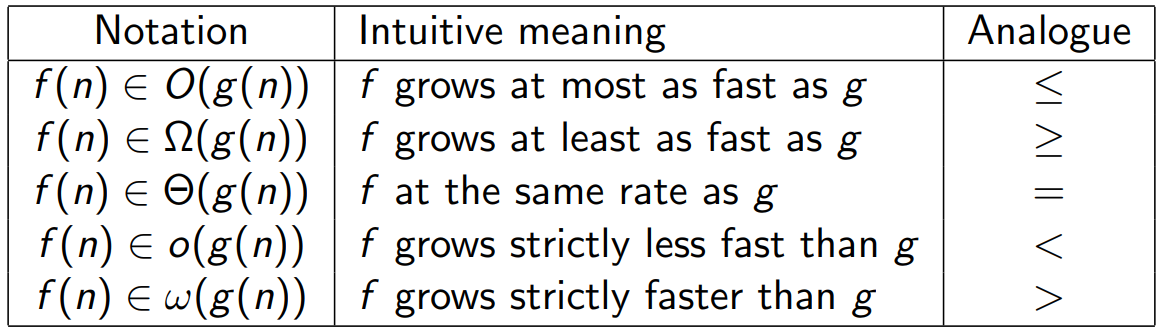
\includegraphics[width=8cm]{big-o-definition.png}
        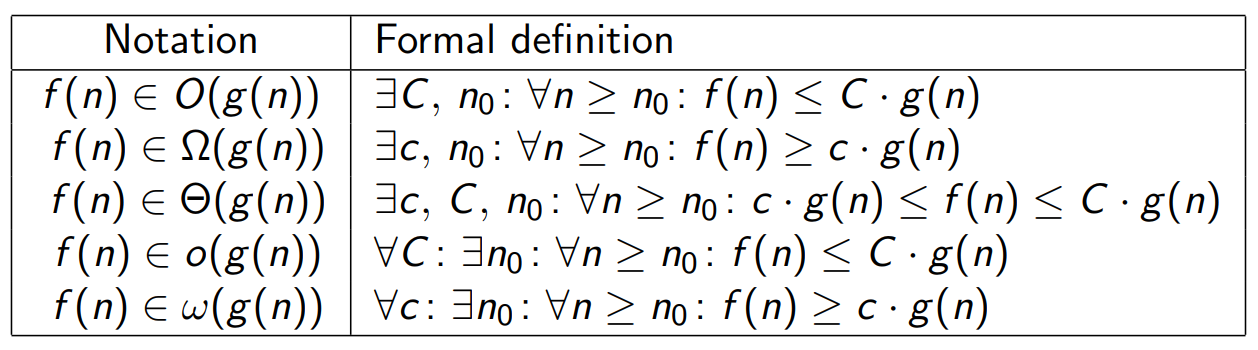
\includegraphics[width=8cm]{big-o-formal.png}
    \end{minipage}
};
%------------ Big O Header ---------------------
\node[fancytitle, right=10pt] at (box.north west) {Big O};
\end{tikzpicture}

%------------ Interval Scheduling ---------------
\begin{tikzpicture}
\node [mybox] (box){%
    \begin{minipage}{0.3\textwidth}
    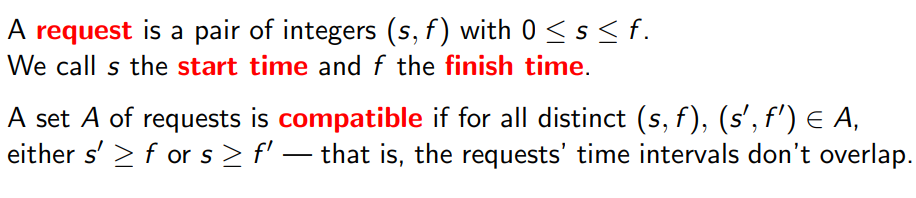
\includegraphics[width = 8cm]{req-comp-def.png}
    \hline
    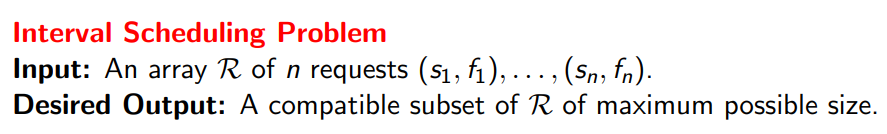
\includegraphics[width = 8cm]{interval-scheduling-problem.png}
    \hline
    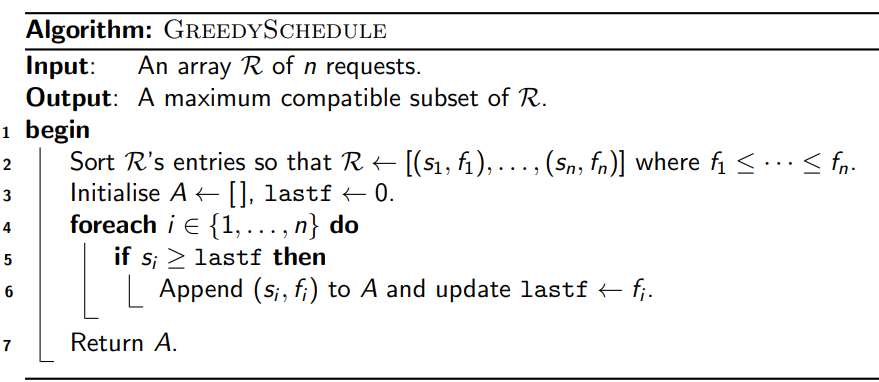
\includegraphics[width=8cm]{greedy-schedule-pseudo.png}
    \textbf{Complexity:} \\
    Step 2 takes O(n log n) \\
    Steps 3–6 all take O(1) time and are executed at most n times. \\
    $\therefore total running time = O(n log n) + O(n) · O(1) = O(n log n).$
    \end{minipage}
};
%------------ Interval Scheduling Header ---------------------
\node[fancytitle, right=10pt] at (box.north west) {Interval Scheduling};
\end{tikzpicture}


%------------ Interval Scheduling 2 ---------------
\begin{tikzpicture}
\node [mybox] (box){%
    \begin{minipage}{0.3\textwidth}
    
    \textbf{Formal GreedySchedule} \\
    $A^+$ := argmin $\{f : (s, f ) \in R, A \cup \{(s, f )\}$ is compatible\} for all $A \subseteq R$, \\
    $A_0 := \emptyset,$ \hspace{1cm} $A_{i+1} := A_i \cup \{A_i^+\}$ \\
    t := max\{i: $A_i$ is defined\}\\
    \textbf{Interval Scheduling Proofs} \\
    \textbf{Lemma}: Greedy Schedule always outupts $A_t$ \\
    \textbf{Proof}: By induction form the following loop invariant.
    At the start of the i'th iteration of 4-7: \\
    \vspace{-5mm}
    \setlist{nolistsep}
    \begin{itemize} [noitemsep]
        \item A is equal to $A_t \cap \{(s_1, f1), ..., (s_{i-1}, f_{i-1})\}$
        \item lastf is equal to the latest finish time of any request in A (or 0 if A = [])
    \end{itemize}
    \hline
    \textbf{Lemma}: $A_t$ is a compatible set \\
    \textbf{Proof}: Instant by induction; $A_0$ is compatible, and if $A_i$ is compatible then so is $A_{i+1} = A_i \cup {A^+}$ by the definition of $A_i^+$
    
    \hline
    \textbf{Lemma}: $A_t$ is a maximum compatible subset of the Array $R$ (look in pseudocode) \\
    \textbf{Proof}:\\
    Base case for i = 1: $A_0^+$ is the fastest finishing request in $R$ by definition\\
    Inductive step: Suppose $A_i$ finishes faster than $B_i$. \\
    Let $B_i^+$ be the (i+1)'st fastetst-finishing element of B.
    Since $A_i$ finishes faster than $B_i$, $A_i \cup \{B_i^+\}$ is compatible. Hence by definition, $A_i^+$ exists and finishes no later than $B_i^+$
    \hline
    \textbf{Theorem}: GreedySchedule outputs $A_t$, which is a maximum compatible set. \\
    \textbf{Proof}: putting all of the above proofs together, we prove the theorem.
    \end{minipage}
};
%------------ Interval Scheduling 2 Header ---------------------
\node[fancytitle, right=10pt] at (box.north west) {Interval Scheduling};
\end{tikzpicture}

%------------ Graph Theory ---------------
\begin{tikzpicture}
\node [mybox] (box){%
    \begin{minipage}{0.3\textwidth}
    \textbf{Definitions}: \\
    \textbf{Graph}: G = (V, E) \\
    \textbf{Edge}: E = E(G) is a set of edges contained in $\{\{u,v\}: u,v \in V, u \neq v\}$ \\
    \textbf{Vertex}: V = V(G) is a set of vertices \\
    \textbf{Subgraph}: H = $(V_H, E_H)$ of G is a graph with $V_H \subseteq V$ and $E_H \subseteq E$ \\
    \textbf{Induced Subgraph}: is a subgraph if $E_H = \{e \in E: e \subseteq V_H\}$ \\
    \textbf{Component}: H of G is a maximal connected induced subgraph of G. \\
    \textbf{Degree}: $d (v) = |N (v)|$ \\
    \textbf{Neighbourhood}: $N (v) = \{w \in V: \{v, w\} \in E\}$ \\
    \textbf{Walk}: sequence of vertices $v_0...v_k$ such that $\{v_i, v_{i+1}\} \in E$ for all i $\le$ k-1 \\
    \textbf{Length}: the value of k (see above walk definition) \\
    \textbf{Euler Walk}: a walk that contains every edge in G exactly once. \\
    \textbf{Isomorphism}: two graphs are isomorphic if there is a bijection f: 
    $V_1 \rightarrow V_2$ such that $\{f(u), f(v)\} \in E_2$ if and only if $\{u, v\} \in E_1$ \\
    \textbf{Path}: is a walk in which no vertices repeat \\
    \textbf{Connected}: A graph is connected if any two vertices are joined by a path \\
    \textbf{Digraph}: is a pair G = (V, E), V is a set of vertices and E is a set of edges contained in $\{(u, v): u, v \in V, u \neq v\}$ \\
    \textbf{Strongly connected}: G is .. if for all $u, v \in V$, there is a path from u to v and a path from v to u. \\
    \textbf{Weakly connected}: \\
    \textbf{In-Neighbourhood}: $N^- (v) = \{u \in V(G): (u, v) \in E(G)\}$ \\
    \textbf{Out-Neighbourhood}: $N^+ (v) = \{w \in V(G): (v, w) \in E(G)\}$ \\
    \textbf{Cycle}: is a walk $W = w_0...w_k$ with $ w_0 = w_k$ and $k \ge 3$,
    in which every vertex appears at most once except for $w_0$ and $w_k$ (which appear twice) \\
    \textbf{Hamilton cycle}: is a cycle containing every vertex in the graph \\
    \textbf{k-regular}: a graph is .. if every vertex has degree k\\
    \textbf{Bijection}: \\
    \end{minipage}
};
%------------ Graph Theory Header ---------------------
\node[fancytitle, right=10pt] at (box.north west) {Graph Theory};
\end{tikzpicture}



%------------ Graph Theory 2 ---------------
\begin{tikzpicture}
\node [mybox] (box){%
    \begin{minipage}{0.3\textwidth}

    \textbf{Theorem}: If G has an Euler walk, then either: \\
    \vspace{-5mm}
    \setlist{nolistsep}
    \begin{itemize} [noitemsep]
        \item every vertex of G has even degree; or
        \item all but two vertices $v_0$ and $v_k$ have even degree, and any euler walk must have $v_0$ and $v_k$ as endpoints
    \end{itemize}
    \hline
    \textbf{Theorem}: let G = (V, E) be a digraph with no isolated vertices, and let $U,v \in V$. Then G has an Euler walk 
    from u to v if and only if G is weakly connected and either: \\
    \vspace{-5mm}
    \setlist{nolistsep}
    \begin{itemize} [noitemsep]
        \item u = v and every vertex of G has equal in- and out-degrees; order
        \item $u \neq v, d^+ (u) = d^- (u) + 1, d^- (v) = d^+ (v) + 1$ and every other vertex of G has equal in- and out-degrees
    \end{itemize}
    \hline
    \textbf{Dirac's Theorem}: Let $n \ge 3$. Then any n-vertex graph G with minimum degree at least $\frac{n}{2}$ has a Hamilton cycle. \\
    % \textbf{Proof}: Try to find a long path inductively: start with a trivial one-vertex path and repeatedly extend it. \\ TODO PROOF
    % Suppose G contains a k-vertex path v1 . . . vk for some k ∈ [n − 1]. \\
    % \textbf{Case 1: $k \le \frac{n}{2}$}: then being greedy works. \\
    % In general, $d(v_k) \ge \frac{n}{2} > |\{v_1, ..., v_{k-1}\}|$, so there’s a vertex $v{k+1}$ adjacent to $v_k$ other than $v_1, . . . , v_{k−1}$. 
    % Then $v_1 . . . v_{k+1}$ is a path of length k + 1. 

    \textbf{Handshake lemma}: For any graph \\G = (V, E), $\sum_{v \in V}^{} d(v) = 2|E|$ \\
    \textbf{Proof}: All edges contain two vertices, and eachvertex v is in d(v) edges. Count the number of verted-edge pairs:
    Let $X = \{(v, e) \in V \times E: v \in E\}$. Then $|X| = 2|E|$ and $|X|$ = $\sum_{v \in V}^{}d(v)$, so we're done.
    \hline

    \textbf{Directed Handshake lemma}: For any graph \\G = (V, E), $\sum_{v \in V}^{} d^+(v) = \sum_{v \in V}^{} d^-(v) = 2|E|$ \\
    \textbf{Proof}: TODO. Instead of counting vertex-edge pairs, we count tail-edge pairs. Each edge has one tail so $|X| = |E|$
    \hline


    \end{minipage}
};
%------------ Graph Theory 2 Header ---------------------
\node[fancytitle, right=10pt] at (box.north west) {Graph Theory};
\end{tikzpicture}


%------------ Trees ---------------
\begin{tikzpicture}
\node [mybox] (box){%
    \begin{minipage}{0.3\textwidth}
    \textbf{Definitions}: \\
    \textbf{Forest}: a graph with no cycles \\
    \textbf{Tree}: a forest that is connected \\
    \textbf{Root}: for T = (V, E). Root $r \in V$ as follows. For all vertices $v \neq r$, let $P_v$ be the unique path from r to v.
    Then direct each $P_v$ from r to v. \\
    \textbf{Leaf}: is a degree-1 vertex. Root cannot be a leaf. \\
    \textbf{Ancestor}: u is an .. of v if u i on $P_v$ \\
    \textbf{Parent}: u is the .. of v if $u \in N^-(v)$ \\
    \textbf{level}: first .. $L_0$ of T is {r}, and $L_{i+1} = N^+(L_i)$. \\
    \textbf{depth}: of T is max\{i: $L_i \neq \emptyset$\}. Root doesn't count  \\
    \hline
    \textbf{Lemma 1}: If T = (V, E) is a tree, then any pair of vertices u, v $\in$ V is joined by a unique path uTv in T. \\
    % \textbf{Proof}: TODO \\
    \textbf{Lemma 2}: Any n-vertex tree has n-1 edges \\
    % \textbf{Proof}: TODO \\
    \textbf{Lemma 3}: Any n-vertex tree T = (V, E) with $n \ge 2$ has at least 2 leaves \\
    % \textbf{Proof}: TODO \\
    \textbf{Tree Properties}: \\
    \textbf{A}: T is connected and has no cycles \\
    \textbf{B}: T has n-1 edges and is connected \\
    \textbf{C}: T has n-1 edges and has no cycles \\
    \textbf{D}: T has a unique path between any pair of vertices \\
    $A \implies B, C, D \hspace{2cm} A \impliedby B, C, D$. \\
\end{minipage}
};
%------------ Trees Header ---------------------
\node[fancytitle, right=10pt] at (box.north west) {Trees};
\end{tikzpicture}



\end{multicols*}
\end{document}